\section{Proof of concept implementation for health data sharing}
\label{sec:poc_health}

In this Section, a proof of concept implementation of the proposed algorithms for offer instantiation and policy matching towards the generation of a data access agreement is described for a specific use case involving health data sharing.

\subsection{Background \& Motivation}
\label{sec:poc_background}

In this Thesis, a health data sharing use case was selected to showcase the strengths of the proposed algorithm since the exchange of health-related data presents significant potential for advancing research and leveraging advanced computational and statistical techniques to drive progress in healthcare.
However, due to its sensitive nature and potentially significant impact if misused, the sharing and utilisation of health-related data are highly regulated at both legal and institutional levels, e.g., \textit{``data concerning health''} is a special category of personal data under the GDPR, i.e., Article 9.1~\citeyearpar{noauthor_regulation_2016}, and as such its processing is prohibited unless one of the legal grounds of Article 9.2 applies.

Currently, institutions such as hospitals handle each health data request through a dedicated committee tasked with evaluating and making decisions regarding the release of such data under their care.
To facilitate this process, the Global Alliance for Genomics and Health\footnote{\url{https://www.ga4gh.org/} (accessed on 2 April 2024)} (GA4GH) was established as an international consortium focused on the development of standards and the promotion of responsible sharing of genomics and health data.
Among its various resources, aimed at different aspects and processes of health-related data sharing, GA4GH has introduced a machine-readable ontology known as the Data Use Ontology\footnote{\url{http://purl.obolibrary.org/obo/duo} (accessed on 2 April 2024)} (DUO).
DUO~\citep{lawson_data_2021,rehm_ga4gh_2021} was designed to express Data Use Limitations (DULs), i.e., conditions and constraints defined by data providers which should be respected by data requesters to use said data.

DUO is an OWL ontology aligned with the Open Biological and Biomedical Ontology\footnote{\url{https://obofoundry.org/} (accessed on 2 April 2024)} (OBO).
By utilising OBO's upper level ontologies, DUO ensures semantic interoperability with a range of biomedical ontologies belonging to the OBO family of ontologies.
As such, DUO's main purpose is related to annotating datasets with DUL codes to specify usage conditions, articulate data usage requests, and automatically identify or discover compatible datasets by comparing requests with datasets' usage conditions.

\paragraph{DUO and existing efforts}
DUO concepts are organised into three taxonomies:
\begin{enumerate}
    \item The `Data Use Permission' taxonomy, denoted by the base class \texttt{obo:DUO\_0000001}, encompasses permissions related to purposes for data usage.
    \item The `Data Use Modifier' taxonomy, denoted by the base class \texttt{obo:DUO\_0000017}, covers additional conditions to be applied alongside data use permissions.
    \item The `Investigation' taxonomy, denoted by the base class \texttt{obo:OBI\_0000066} from the Ontology for Biomedical Investigations\footnote{\url{http://obi-ontology.org/} (accessed on 3 April 2024)} (OBI), delineates planned conditions for which data is being requested.
\end{enumerate}
Furthermore, the \texttt{obo:DUO\_0000010} property implements a \textit{`is restricted to'} relation, used to limit certain concepts to certain contexts, e.g., to restrict the \texttt{obo:DUO\_0000022} concept, which indicates usage permitted within a geographic region, to terms from \texttt{obo:GAZ\_00000448}, the base concept from the Gazetteer (places) ontology\footnote{\url{https://environmentontology.github.io/gaz/} (accessed on 3 April 2024)}.

DUO originated from prior endeavours aimed at establishing consent codes for data usage and leveraging them as machine-readable information for automated access to data.
Its initial development drew upon the Consent Codes by \cite{dyke_consent_2016}, which specified concepts for data usage based on consent permissions.
Subsequently, DUO incorporated a few terms from the Automatable Discovery and Access Matrix (ADA-M) framework \citep{woolley_responsible_2018}, which shares akin objectives and concepts.
As such, the intended utilisation of DUO revolves around facilitating the recording of consent for sharing and reusing biomedical datasets, as outlined by \cite{lawson_data_2021} and \cite{rehm_ga4gh_2021}, the latter highlighting the usage of DUO in distinct GA4GH initiatives.

The Data Use Oversight System\footnote{\url{https://duos.broadinstitute.org/} (accessed on 2 April 2024)} (DUOS) is a platform built upon DUO aimed at facilitating semi-automated management of access health-related datasets.
It leverages DUO annotations to incorporate new datasets and data access requests, which are subsequently matched using an algorithm based on hierarchical compatibility.
Figure~\ref{fig:duo-matching} illustrates the algorithm followed by this platform, where the `Data Use Codes' correspond to concepts from the previously mentioned DUO `Data Use Permission' taxonomy,  the `Data Use Requirements' to the `Data Use Modifier' taxonomy, and the `Research Purpose Terms/Data Use Categories' to the `Investigation' taxonomy.
This algorithm entails matching the dataset's access conditions with the data requester's conditions by relying on the subclass relations between them.
The results of this matching algorithm are then reviewed by a `Data Access Committee' to finalise the conditions of the access agreement and provide the data requested with access to the relevant datasets, comparable with the decision-making processes of human data access committees \citep{cabili_empirical_2021}.
The NHGRI Genomic Data Science Analysis, Visualization, and Informatics Lab-space project\footnote{\url{https://anvilproject.org} (accessed on 3 April 2024)} implemented a large-scale pilot using the DUOS platform implementation \citep{schatz_inverting_2022}.

Beyond DUOS, the DUO specification has been integrated into various other works, including a specification of informed consent for health and genomics research in Africa \citep{nembaware_framework_2019}, a blockchain-based consent model for health data sharing \citep{jaiman_consent_2020}, and an online platform that offers dynamic consent interfaces and tools for large-scale genomics research programs \citep{haas_ctrl_2021}.
Furthermore, DUO is mentioned in the Data Tags Suite (DATS), where it is considered a candidate vocabulary within its framework for discovering metadata-based data access conditions \citep{alter_data_2020}.
Additionally, it plays a role in the roadmap of European infrastructures for accessing a large number of human genomes  \citep{saunders_leveraging_2019}.
Moreover, \cite{amith_expressing_2022} demonstrate the usage of DUO for the representation of consent metadata, employing SWRL\footnote{\url{https://www.w3.org/Submission/SWRL/} (accessed on 3 April 2024)} to execute permissive rules, and \cite{grabus_landscape_2019} provide a comprehensive overview of rights and licensing initiatives, approaches, and tools for health data sharing, including DUO.

\paragraph{Challenges of the DUO specification}
DUO expresses DULs as concepts with human-readable definitions, utilising the \texttt{obo:IAO\_0000115} property, e.g., as \texttt{skos:definition} is used to define SKOS concepts.
This limits their utility to humans or machines that operate solely on known concepts.
Furthermore, DUO concepts lack linkage to relevant legal concepts, leading to ambiguity regarding the implications of their usage in strongly legislated jurisdictions like the EU, where the GDPR~\citeyearpar{noauthor_regulation_2016} introduces additional accountability and compliance requirements that must be acknowledged and adhered to.
While existing documentation mentions that the applicability of laws falls under the responsibility of the adopter and that DUO terms have not been evaluated for GDPR compliance, it is crucial for data subjects and data controllers to ensure compatibility with existing regulations.
As such, the absence of such support from the DUO specification poses a risk of hindering interoperability as additional approaches need to be taken to fulfil legal requirements.
Moreover, with the EU push to have a common `Health Data Space'\footnote{\url{https://ec.europa.eu/health/ehealth-digital-health-and-care/european-health-data-space_en} (accessed on 2 April 2024)}, machine-readability and automation will play a pivotal role in facilitating legally-aligned health data exchange.

Furthermore, no instructions were found on how to associate DUO conditions with datasets nor on how the data access agreements matching algorithm should work.
While the DUOS framework provides a comprehensive description of how DUO can be utilised, it lacks detailed guidance on the matching algorithm.
DATS \citep{alter_data_2020} also acknowledges the challenge of using DUO for defining permissions and prohibitions, suggesting ODRL as an alternative model for clearer articulation of permissions and prohibitions.

\paragraph{Proposed improvements over the DUO specification}
To achieve \textit{true machine-readability}, DUO concepts must be represented with permissions, prohibitions, constraints, and duties to form machine-readable rules, by leveraging semantic standards for the expression of asset usage conditions.
By formalising the DULs embedded within the descriptions of each DUO concept as a set of rules, these become explicit and can be attached and sent alongside the data for future inspection.

To assess the compatibility of a data request with the dataset's DULs, both the conditions set by the data provider and those articulated by the data requester for data use should be formulated as policies.
These policies can then be matched to determine if the intended use aligns with the dataset's conditions, using the same approach as the one presented in Section~\ref{sec:algorithm}.
While DUO is currently being utilised in this manner, as evidenced in systems like DUOS, the matching relies on hierarchical compatibility between data request and data use conditions established through a subclass relationship, i.e., a data request $DR$ is a subclass/superclass of a data use condition $DUC$.
This approach has limitations in terms of its capacity and expressiveness for delineating fine-grained rules to utilise in automated systems, as not all relevant pieces of information can be explicitly captured in distinct concepts.
For instance, DUO's \texttt{DUO\_0000006} indicates through a sole human-readable label that use is allowed for health/medical/biomedical research purposes, not including the study of population origins or ancestry, while the same information can be much more explicitly declared using ODRL policies with permission and prohibition rules with purpose constraints.

More significantly, in order to automate the generation of data access/usage agreements effectively, a set of criteria should be considered when selecting a vocabulary to articulate such conditions:
\begin{enumerate}
    \item[(i)] the level of expressiveness to define rules and policies, encompassing the ability to express actions, purposes, or other constraints as distinct concepts that can be autonomously specified and evaluated, and combined in distinct ways to represent various types of policies;
    \item[(ii)] the capability to associate and verify their conformity and adherence to legal requirements, e.g., such as the GDPR; and
    \item[(iii)] the capacity to specify access/usage conditions in a machine-readable format and utilise them for assessing the accuracy and comprehensiveness of information that should be in such a data agreement.
\end{enumerate}
% FROM THE PAPER: Such solutions have existed for a while now -- for example, Answer Set Programming (ASP) and logic-based semantic reasoners have been utilised in a variety of domains -- including for representing information and using it for checking legal compliance for GDPR (see Section.\ref{sec:sota-legal}).

With the aforementioned motivation in mind, this Thesis proposes an approach to explicitly represent DUO concepts using RDF, leveraging ODRL and the efforts declared in previous Sections related with an OAC-based architecture for decentralised access to data.
The choice of using ODRL, beyond being a W3C Recommendation for the expression of policies, is supported by the following motives:
\begin{enumerate}
    \item[(i)] it is RDF-based, ensuring machine-readability;
    \item[(ii)] it encompasses concepts that model domain-specific and legally relevant terms to depict constraints, such as spatial and temporal operators, as well as support various types of policies like offers, requests, and agreements; % Additionally, it offers flexibility in utilizing these concepts in a manner analogous to the conventional contents and structures of legal agreements;
    \item[(iii)] its usage can be validated, and efforts are underway within the W3C ODRL CG to actively develop a formal semantics specification~\citep{fornara_odrl_2023};
    \item[(iv)] it facilitates the development of extensions through ODRL profiles, offering the flexibility to tailor ODRL to specific requirements -- as proved by this Thesis' work on OAC (Section~\ref{sec:oac}), which connects ODRL with legal requirements using DPV and can be extended to cater for legal requirements of health data sharing; and
    \item[(v)] backwards compatibility can be ensured -- existing DUO-based systems can adopt the practices suggested in this Section and continue being compatible with the DUO specification. Also, DUO users can select which aspects of this solution they want to incorporate in their system.
\end{enumerate}

As such, based on the algorithms described in Section~\ref{sec:algorithm}, in this Section, (i) DUO concepts are modelled as ODRL policies, (ii) such policies are instantiated as ODRL offers for the access to health-related datasets, (iii) offers are matched with incoming data requests to generate permissive or prohibitive data agreements, and (iv) work on OAC is recycled to deal with GDPR obligations for the processing of health data.

\begin{figure}[ht]
    \centering
    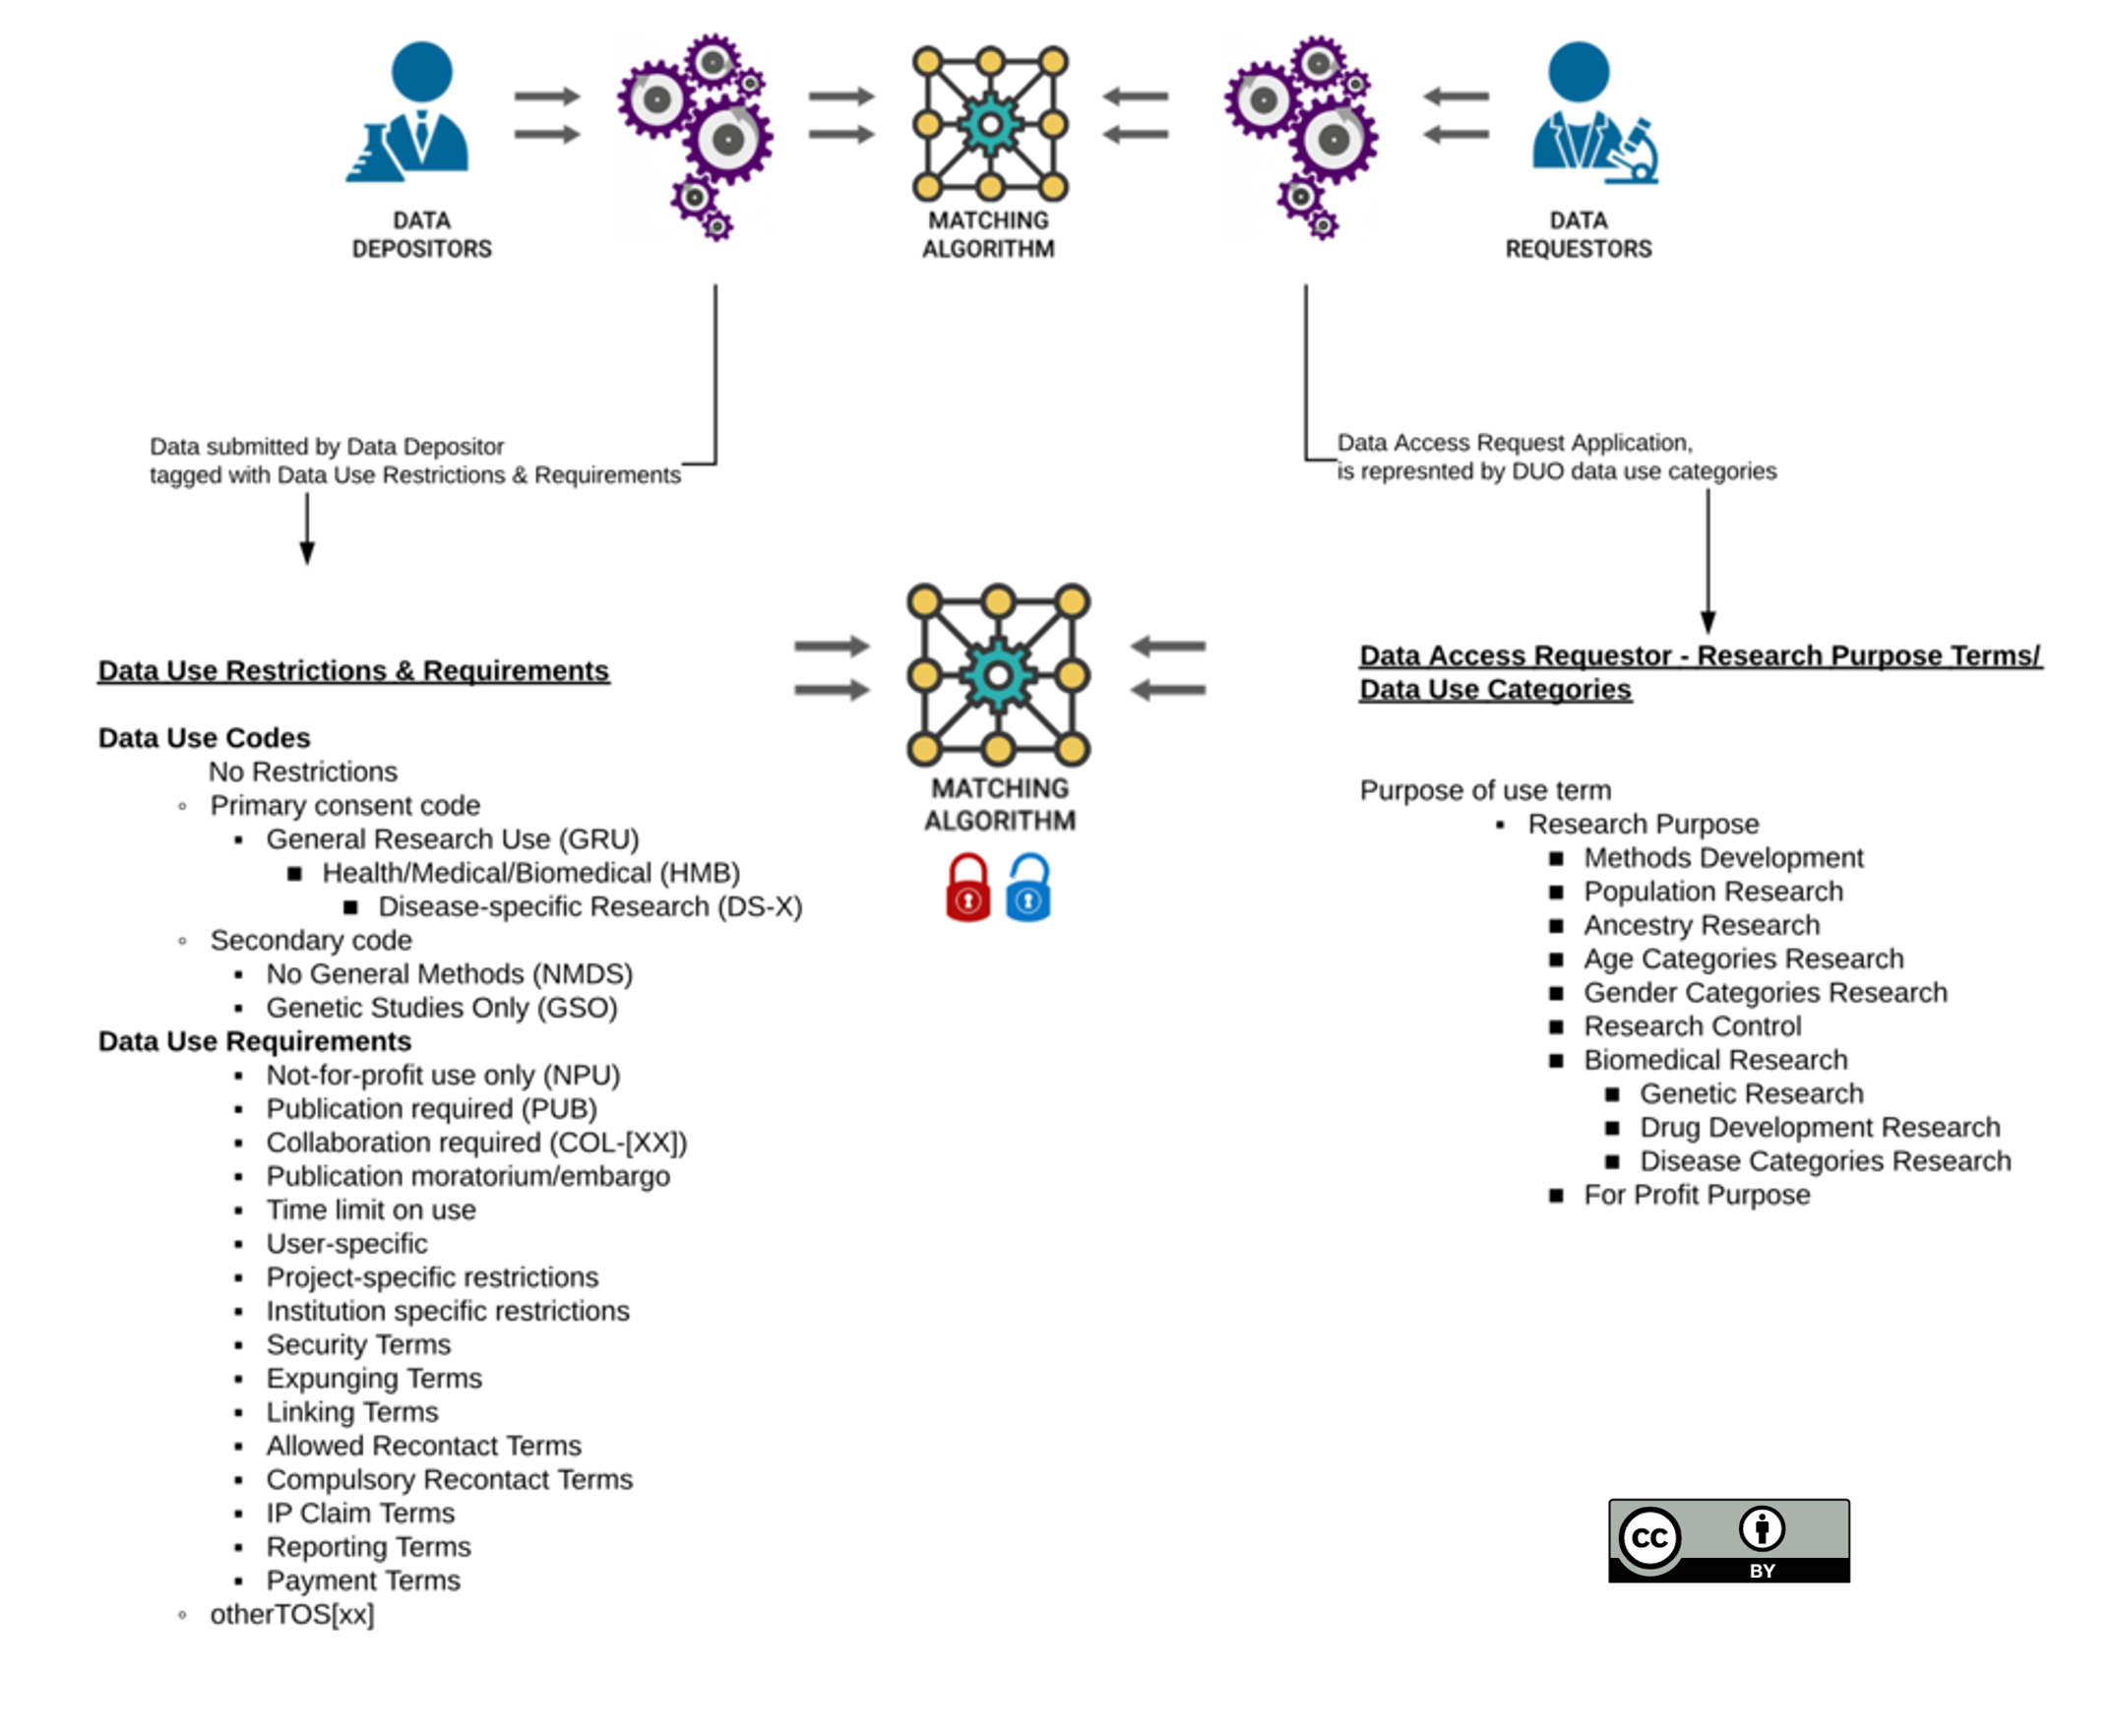
\includegraphics[width=1\linewidth]{figures//chapter-6/DUO-matching-with-license.png}
    \caption{DUO-based matching algorithm, adapted from \url{https://github.com/EBISPOT/DUO}.}
    \label{fig:duo-matching}
\end{figure}

% modelling of DUODRL
% extension of the policy matching algorithm to deal with DUODRL requirements
% poc implementation